\documentclass{article}

\usepackage{graphicx}
\usepackage{tikz}
\usepackage{tikzsymbols}
\usetikzlibrary{calc,patterns,shapes.geometric}
\pagestyle{empty}
\usepackage[margin=0pt]{geometry}
\geometry{papersize={14in,12in}}

\def\centerarc[#1](#2)(#3:#4:#5){\draw[#1] ($(#2)+({#5*cos(#3)},{#5*sin(#3)})$) arc (#3:#4:#5);}

\begin{document}
	\begin{figure}
		\centering
		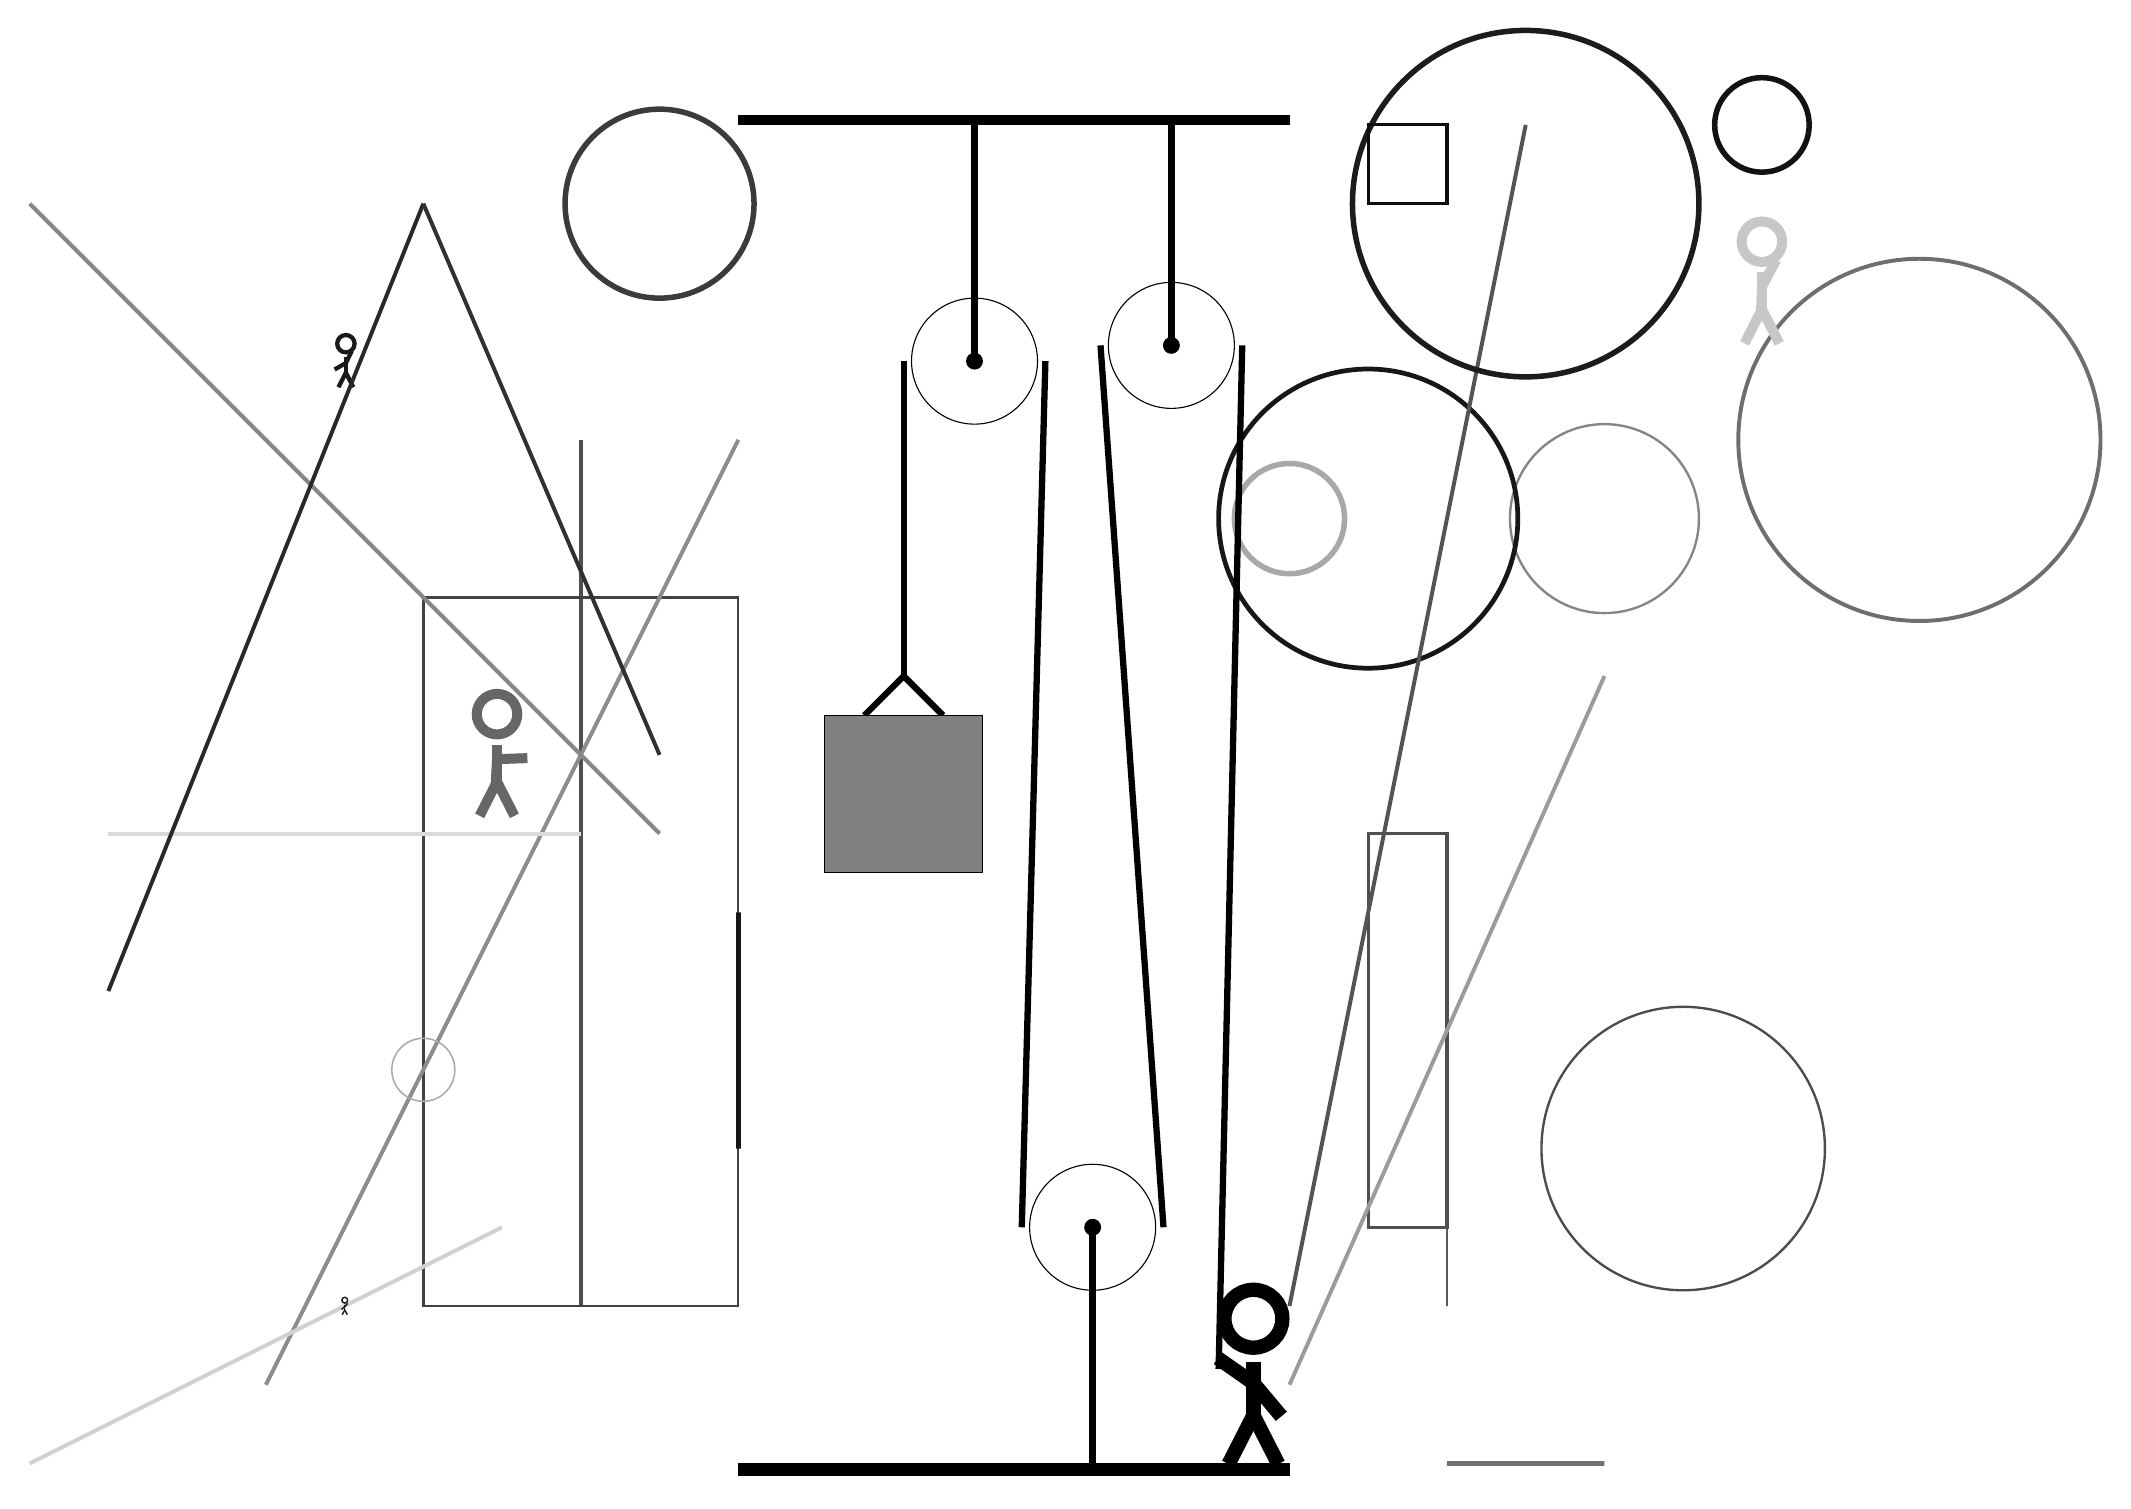
\begin{tikzpicture}
			%%%%% START %%%%%
			
			\draw[fill=black] (-2, 14) rectangle (5, 14.125);
			
			\draw (1, 11) circle (0.8);
			\draw[fill=black] (1, 11) circle (0.1);
			\draw[line width=0.8mm]  (1, 14) -- (1, 11);
			
			\draw[fill=white](2.5, 0) circle (0.8);
			\draw[fill=black] (2.5, 0) circle (0.1);
			\draw[line width=0.8mm]  (2.5, -3) -- (2.5, 0);
			
			\draw[fill=white](3.5, 11.2) circle (0.8);
			\draw[fill=black] (3.5, 11.2) circle (0.1);
			\draw[line width=0.8mm] (3.5, 14) -- (3.5, 11.2);
			
			\draw [line width=0.5mm, color=black!57](13, 10) circle (2.3);
			
			\draw [line width=0.7mm, color=black!77](-3, 13) circle (1.2);
			\draw[line width=0.5mm, color=black!69](-4, 10) -- (-4, -1);
			\draw[line width=0.3mm, color=black!74] (-2, -1) rectangle (-6, 8);
			
			\draw[line width=0.5mm, color=black!45](-2, 10) -- (-8, -2);
			
			\draw [line width=0.7mm, color=black!34](5, 9) circle (0.7);
			\draw[line width=0.3mm, color=black!65] (7, -1) rectangle (7, 3);
			\draw[line width=0.4mm, color=black!69] (7, 0) rectangle (6, 5);
			\draw[line width=0.5mm, color=black!14](-4, 5) -- (-10, 5);
			
			\draw [line width=0.2mm, color=black!33](-6, 2) circle (0.4);
			
			\node[line width=0.5mm, color=black!90] at (-7, 11) {\Strichmaxerl[3][30][64]};
			
			\node[line width=0.4mm, color=black!22] at (11, 12) {\Strichmaxerl[7][88][62]};
			\draw[line width=0.5mm, color=black!18](-5, 0) -- (-11, -3);
			\draw [line width=0.3mm, color=black!48](9, 9) circle (1.2);
			\draw[line width=0.5mm, color=black!39](9, 7) -- (5, -2);
			\draw[line width=0.7mm, color=black!91] (-2, 4) rectangle (-2, 1);
			
			\node[line width=0.7mm, color=black!60] at (-5, 6) {\Strichmaxerl[7][87][2]};
			\draw[line width=0.5mm, color=black!47](-3, 5) -- (-11, 13);
			\draw[line width=0.6mm, color=black!56] (7, -3) rectangle (9, -3);
			\draw [line width=0.6mm, color=black!91](6, 9) circle (1.9);
			\draw[line width=0.5mm, color=black!84](-6, 13) -- (-10, 3);
			
			\draw[line width=0.5mm, color=black!81](-3, 6) -- (-6, 13);
			\node[line width=0.2mm, color=black!90] at (-7, -1) {\Strichmaxerl[1][42][48]};
			\draw[line width=0.5mm, color=black!67](5, -1) -- (8, 14);
			\draw [line width=0.3mm, color=black!70](10, 1) circle (1.8);
			
			\draw [line width=0.7mm, color=black!89](8, 13) circle (2.2);
			\draw [line width=0.7mm, color=black!93](11, 14) circle (0.6);
			\draw[line width=0.4mm, color=black!95] (7, 13) rectangle (6, 14);
			
			
			\draw[line width=0.8mm] (-0.4, 6.5) -- (0.1, 7.0) -- (0.6, 6.5);
			\draw[fill=black!50] (-0.9, 6.5) rectangle (1.1, 4.5);
			
			\draw[line width=0.8mm] (0.1, 11) -- (0.1, 7.0);
			\centerarc[line width=0.8mm](1, 11)(0:180:0.9);
			\draw[line width=0.8mm](1.9, 11) -- (1.6, 0);
			\centerarc[line width=0.8mm](2.5, 0)(180:360:0.9);
			\draw[line width=0.8mm](3.4, 0) -- (2.6, 11.2);
			\centerarc[line width=0.8mm](3.5, 11.2)(0:180:0.9);
			\draw[line width=0.8mm](4.4, 11.2) -- (4.1, -1.8);
			
			\node at (4.5, -1.9) {\Strichmaxerl[10][-35][-50]};
			
			\draw[fill=black] (-2, -3) rectangle (5, -3.15);
			
			%%%%% END %%%%%
		\end{tikzpicture}
	\end{figure}	
\end{document}